
%%%%%%%%%%%%%%%%%%%%%%%%%%%%%%%%%%%%%%%%%%%%%%%%%%%%%%%%%%
%%
%% This is the "PREAMBLE". Here we define the type of document and load in any packages we might want. You can also set parameters %% % and create your own short-hand here.
%%
%%%%%%%%%%%%%%%%%%%%%%%%%%%%%%%%%%%%%%%%%%%%%%%%%%%%%%%%%%

 \documentclass[9pt]{article}

 \def\solutions{1}
 \usepackage{xcolor}
 \usepackage{amsmath}
 \usepackage{amssymb}
 \usepackage{graphicx}    % needed for including graphics e.g. EPS, PS \usepackage{tikz}
 \usepackage{tikz}\usetikzlibrary{calc,arrows.meta}
 \usepackage{tikz-qtree}
 \usepackage{tikzsymbols}
 \usepackage{relsize}
 \usetikzlibrary{patterns,decorations.pathreplacing,shapes,arrows}
 \usepackage{algorithm2e}
 \topmargin -2.5cm        % read Lamport p.163
 \oddsidemargin -0.04cm   % read Lamport p.163
 \evensidemargin -0.04cm  % same as oddsidemargin but for left-hand pages
 \textwidth 16.59cm
 \textheight 25.94cm
% \pagestyle{empty}        % Uncomment if don't want page numbers
 \pagenumbering{gobble}
 \parskip 7.2pt           % sets spacing between paragraphs
 %\renewcommand{\baselinestretch}{1.5} 	% Uncomment for 1.5 spacing between lines
 \parindent 0pt		  % sets leading space for paragraphs

% No date in header
\date{}

\usepackage{hyperref}
\hypersetup{
    colorlinks=true,
    linkcolor=blue,
    filecolor=magenta,
    urlcolor=cyan,
}
\usepackage{amsthm}
\usepackage{fancyhdr}
\pagestyle{fancy}
\setlength{\headsep}{36pt}

\usepackage{hyperref}

\newcommand{\lp}{\left(}
\newcommand{\rp}{\right)}
\newcommand{\lb}{\left[}
\newcommand{\rb}{\right]}
\newcommand{\ls}{\left\{}
\newcommand{\rs}{\right\}}
\newcommand{\lbar}{\left|}
\newcommand{\rbar}{\right|}
\newcommand{\ld}{\left.}
\newcommand{\rd}{\right.}

\newcommand{\myexists}{\exists \hspace{.3mm}}

\newcommand{\hs}{\hspace{.75mm}}
\newcommand{\bs}{\hspace{-.75mm}}
\newcommand{\nin}{\noindent}

\newcommand{\fx}{f\bs\left( x \right)}
\newcommand{\gx}{g\bs\left( x \right)}
\newcommand{\qx}{q\bs\left( x \right)}

\newcommand{\nn}{\nonumber}

\newcommand{\vfive}{\vspace{5mm}}
\newcommand{\vthree}{\vspace{3mm}}

\newcommand{\fof}[1]{f\lp #1\rp}
\newcommand{\gof}[1]{g\lp #1\rp}
\newcommand{\qof}[1]{q\lp #1\rp}

\newcommand{\myp}[1]{\left( #1 \right)}
\newcommand{\myb}[1]{\left[ #1 \right]}
\newcommand{\mys}[1]{\left\{ #1 \right\}}
\newcommand{\myab}[1]{\left| #1 \right|}

\newcommand{\myj}{_j}
\newcommand{\myjp}{_{j+1}}
\newcommand{\myjm}{_{j-1}}

\newcommand{\f}[1]{f\hspace{-1mm}\left( #1 \right)}
\newcommand{\fp}[1]{f'\hspace{-1mm}\left( #1 \right)}
\newcommand{\g}[1]{g\hspace{-1mm}\left( #1 \right)}
\newcommand{\gp}[1]{g'\hspace{-1mm}\left( #1 \right)}
\newcommand{\q}[1]{q\hspace{-1mm}\left( #1 \right)}
\newcommand{\qp}[1]{q'\hspace{-1mm}\left( #1 \right)}
\newcommand{\Px}[1]{P\hspace{-1mm}\left( x_{#1} \right)}
\newcommand{\Qx}[1]{Q\hspace{-1mm}\left( x_{#1} \right)}

\newcommand{\tten}[1]{\times 10^{#1}}

\newcommand{\aij}[1]{a_{#1}}
\newcommand{\bij}[1]{b_{#1}}
\newcommand{\rij}[1]{r_{#1}}

\newcommand{\R}[1]{\mathbb{R}^{#1}}

\newcommand{\ith}{i^{\textrm{th}}}
\newcommand{\jth}{i^{\textrm{th}}}
\newcommand{\kth}{i^{\textrm{th}}}

\newcommand{\inv}[1]{{#1}^{-1}}

\newcommand{\bx}{\mathbf{x}}
\newcommand{\bv}{\mathbf{v}}
\newcommand{\bw}{\mathbf{w}}
\newcommand{\by}{\mathbf{y}}
\newcommand{\bb}{\mathbf{b}}
\newcommand{\be}{\mathbf{e}}
\newcommand{\br}{\mathbf{r}}
\newcommand{\xhat}{\hat{\mathbf{x}}}

\newcommand{\beq}{\begin{eqnarray}}
\newcommand{\eeq}{\end{eqnarray}}

\newcommand{\ben}{\begin{enumerate}}
\newcommand{\een}{\end{enumerate}}

\newcommand{\bsq}{\mathsmaller{\blacksquare}}

\newcommand{\iter}[1]{^{\myp{#1}}}

% matrix macro
\newcommand{\mymat}[1]{
\left[
\begin{array}{rrrrrrrrrrrrrrrrrrrrrrrrrrrrrrrrrrrrrrr}
#1
\end{array}
\right]
}

\newcommand{\makenonemptybox}[2]{%
%\par\nobreak\vspace{\ht\strutbox}\noindent
\item[]
\fbox{% added -2\fboxrule to specified width to avoid overfull hboxes
% and removed the -2\fboxsep from height specification (image not updated)
% because in MWE 2cm is should be height of contents excluding sep and frame
\parbox[c][#1][t]{\dimexpr\linewidth-2\fboxsep-2\fboxrule}{
  \hrule width \hsize height 0pt
  #2
 }%
}%
\par\vspace{\ht\strutbox}
}
\makeatother

\newcommand{\smallaug}[1]{
\left[
\begin{array}{rr|r}
#1
\end{array}
\right]
}

\tikzset{
	vertex/.style={circle,draw,minimum size=16, inner sep=0pt,font=\normalsize},
	every node/.style={draw=none,rectangle,font=\scriptsize,outer sep=0pt,inner sep=2pt},
	directed/.style={arrows={-Stealth[length=7pt]},font=\small},
	caption/.style={text width=6cm,align=center,rectangle,draw}
	}
\newcounter{dummy}
\newcommand\myitem[1][]{\item[#1]\refstepcounter{dummy}\def\@currentlabel{#1}}

%%%%%%%%%%%%%%%%%%%%%%%%%%%%%%%%%%%%%%%%%%%%%%%%%%%%%%%%%%
%%
%% End of PREAMBLE
%%
%%%%%%%%%%%%%%%%%%%%%%%%%%%%%%%%%%%%%%%%%%%%%%%%%%%%%%%%%%

\newcommand*\circled[1]{\tikz[baseline=(char.base)]{
            \node[shape=circle,draw,inner sep=2pt] (char) {#1};}}

% ======================================================================================
% Actual document starts here.
% PLEASE FILL IN YOUR NAME AND STUDENT ID.
% ======================================================================================
\begin{document}

\lhead{{\bf CSCI 3104, Algorithms \\ Problem Set 9 (50 points)} }
\rhead{Name: \fbox{Jaryd Meek}  \\  ID: \fbox{} \\ Collaborators: Noah Nguyen, Emily Parker \\ {\bf Due April 2, 2021 \\ Spring 2021, CU-Boulder}}
\renewcommand{\headrulewidth}{0.5pt}

\phantom{Test}

\begin{small}
\textit{Advice 1}:\ For every problem in this class, you must justify your answer:\ show how you arrived at it and why it is correct. If there are assumptions you need to make along the way, state those clearly.
\vspace{-3mm}

\textit{Advice 2}:\ Verbal reasoning is typically insufficient for full credit. Instead, write a logical argument, in the style of a mathematical proof.\\
\vspace{-3mm}

\textbf{Instructions for submitting your solution}:
\vspace{-5mm}

\begin{itemize}
	\item The solutions \textbf{should be typed} and we cannot accept hand-written solutions. \href{http://ece.uprm.edu/~caceros/latex/introduction.pdf}{Here's a short intro to Latex.}
	\item You should submit your work through \href{https://www.gradescope.com/courses/218966}{\textbf{Gradescope}} only.
	\item The easiest way to access Gradescope is through our Canvas page. There is a Gradescope button in the left menu.
	\item Gradescope will only accept \textbf{.pdf} files.
	\item \href{https://www.youtube.com/watch?v=u-pK4GzpId0&feature=emb_logo}{It is vital that you match each problem part with your work.} Skip to 1:40 to just see the matching info.
\end{itemize}
\vspace{-4mm}
\end{small}

\hrulefill
\pagebreak

\phantom{Test}

\ben
%%%%%%%%%%%%%%%%%%%%%%%%%%%%%%%%%%%%%%%%%%%%%%%%%%%%%%%%
% PROBLEM  ONE %% PROBLEM  ONE %% PROBLEM  ONE %% PROBLEM  ONE %% PROBLEM  ONE %
%==============================================================================
% Problem 1:minimum spanning tree
%==============================================================================
% PROBLEM  ONE %% PROBLEM  ONE %% PROBLEM  ONE %% PROBLEM  ONE %% PROBLEM  ONE %
%%%%%%%%%%%%%%%%%%%%%%%%%%%%%%%%%%%%%%%%%%%%%%%%%%%%%%%%
\item

Recall that the fibonacci numbers form a sequence wherein each number is the sum of the previous two numbers in the sequence.

\ben
  \item

  Give the recurrence relation for the definition of the fibonacci sequence.

  \item

  Assume you have a program that implements the function $fib(n)$ to compute the $nth$ fibonacci number with the recursive approach. Draw the recursion tree of function calls to compute $fib(4)$ \\

  Tree Example of function $func$ using tikz: \\
  \begin{tikzpicture}[sibling distance=8em,
                      every node/.style = {align=center}]
    \node {func(n)}
      child {
        node {func(n')}
      }
      child {
        node {fun(n'')}
      };
  \end{tikzpicture} \\\\
  *Note if you want to make the tree with a different program, you can simply embed an image of it in the latex submission. A handwritten tree is also acceptable if it is extremely legible.

  \item See the following function that uses a dynamic programming trick to implement $fib(n)$ with a faster runtime than the recursive one. Give the time complexity in terms of $\mathcal{O}()$ for the recursive implementation, as well as for Algorithm. \ref{algo:dynamicFib} below. You do not need to write a proof. Explain why the dynamic programming algorithm is faster.

  \begin{center}
  \begin{algorithm}
    \SetKwProg{Def}{def}{:}{}\Def{fib(n)} {
      {$memo \gets [0,1]$}\;
      \For{$i$ in $2..n$}{
        $memo[i] \gets memo[i-1] + memo[i-2]$\;
      }

      return $memo[n]$
    }
    \caption{Dynamic fibonacci}
    \label{algo:dynamicFib}
  \end{algorithm}
  \end{center}

\een

\if\solutions1
 \vspace{2mm}

 \pagebreak
 \phantom{Test}
 \textbf{Solution:}   \\
%==============================================================================
% STUDENTS: TYPE YOUR SOLUTIONS HERE. (Between \textbf{Solution:} and \fi )
%==============================================================================
\ben
  \item The recurrence relation for the fibonacci sequence is \\
      $U_a(n) = \begin{cases}
        U_a(n-1) + U_a(n-2) & \text{when } n\ge2,\\
        1& \text{when } n=1,\\
        0 & \text{when } n=0.
      \end{cases}$

  \item The recurrence tree for fib(4) is \\
  \begin{tikzpicture}[level distance=1.5cm, level 1/.style={sibling distance=3cm}, level 2/.style={sibling distance=1.5cm}, every node/.style = {align=center}]
      \node {fib(4)}
      child {
        node{fib(3)}
        child{
          node{fib(2)}
          child{node {fib(1)}}
          child{node {fib(0)}}
        }
        child{node {fib(1)}}
      }
      child {
        node{fib(2)}
        child{node {fib(1)}}
        child{node {fib(0)}}
      };
    \end{tikzpicture} \\\\
  

    \item The runtime for $fib(n)$ is \\
      $$\text{Recursive - }\mathcal{O}(2^n)$$
      $$\text{Dynamic - }\mathcal{O}(n)$$
      This is due to the fact that the recursive implementation has to check the same calculation over and over, while the dynamic program calculates it once and stores it. This causes the dynamic implementation to use more memory storing the previous calculations, but means that it operates significantly faster.\\
      As can be seen from the recursion tree above, the recursive implementation has at most $2^n$ nodes, therefore it is $\mathcal{O}(2^n)$
  \een

\fi

\newpage

\phantom{Test}
%%%%%%%%%%%%%%%%%%%%%%%%%%%%%%%%%%%%%%%%%%%%%%%%%%%%%%%%
% PROBLEM TWO %% PROBLEM TWO %% PROBLEM TWO %% PROBLEM TWO %% PROBLEM TWO %
%==============================================================================
% Problem 2: Topic 2
%==============================================================================
% PROBLEM TWO %% PROBLEM TWO %% PROBLEM TWO %% PROBLEM TWO %% PROBLEM TWO %
%%%%%%%%%%%%%%%%%%%%%%%%%%%%%%%%%%%%%%%%%%%%%%%%%%%%%%%%

\vspace{5mm}


\item Consider the Knapsack problem for the list $A = [(4, 3), (1, 2), (3, 1), (5, 4), (6, 3)] $ of (weight, value) pairs. The weight threshold is $W = 10$.

\begin{enumerate}
    \item Fill in the table below using the bottom-up DP algorithm.   


\begin{tabular}{|c|c|||c|c|c|c|c|c|c|c|c|c|c|c|}
\hline
Weight & Value&$w=0$ & 1& 2& 3& 4& 5& 6& 7& 8& 9&10 \\
\hline
-& -& & & & & & & & & & &\\
\hline
4 &3 & & & & & & & & & & &\\
\hline
1 &2 & & & & & & & & & & &\\	
\hline
3 &1 & & & & & & & & & & &\\	
\hline
5 &4 & & & & & & & & & & &\\	
\hline
6 &3 & & & & & & & & & & &\\	
\hline
\end{tabular}
	




    \item Write an algorithm that prints the optimal subset of items once the bottom-up DP algorithm has finished.  Your algorithm should only use the filled in table and the inputs to the bottom-up algorithm. 
    \item Highlight in \textcolor{red}{red} the numbers in each cell that your algorithm from part (b) visits. \circled{\textcolor{red}{Circle}} each cell that is part of the optimal solution. (Indicate this on the same table from part (a).)
    \item  Does the order that we consider the items change the optimal solution? Explain why or why not.


\end{enumerate}

\if\solutions1
\vspace{2mm}

\phantom{test}

\textbf{Solution:} \\
%==============================================================================
% STUDENTS: TYPE YOUR SOLUTIONS HERE. (Between \textbf{Solution:} and \fi )
%==============================================================================
\ben
\item 
\begin{tabular}{|c|c|||c|c|c|c|c|c|c|c|c|c|c|c|}
  \hline
  Weight & Value&$w=0$ & 1& 2& 3& 4& 5& 6& 7& 8& 9&10 \\
  \hline
  -& -&0 &0 &0 &0 &0 &0 &0 &0 &0 &0 &0\\
  \hline
  4 &3 &0 &0 &0 &0 &\circled{\textcolor{red}{3}} &3 &3 &3 &3 &3 &3\\
  \hline
  1 &2 &0 &2 &2 &2 &3 &\circled{\textcolor{red}{5}} &5 &5 &5 &5 &5\\	
  \hline
  3 &1 &0 &2 &2 &2 &3 &\textcolor{red}{5} &5 &5 &6 &6 &6\\	
  \hline
  5 &4 &0 &2 &2 &2 &3 &5 &6 &6 &6 &7 &\circled{\textcolor{red}{9}}\\	
  \hline
  6 &3 &0 &2 &2 &2 &3 &5 &6 &6 &6 &7 &\textcolor{red}{9}\\	
  \hline
  \end{tabular}

  \item The following is written in Python.\\
  Inputs to the function - \\ Chart is a 2d array of the chart after the bottom-up DP algorithm has finished.\\ Items is a 2d array of the weights and their values in the form [[weight, value],[weight, value]]
    \begin{verbatim}
  def knapsack(chart, items): 
      output = []
      x = len(chart[0]) - 1
      y = len(chart) - 1
      while y > 0:  
          if chart[y-1][x] < chart[y][x]: 
              x -= items[y-1][0]
              output.append(items[y-1])
          y -= 1
      print(output)
    \end{verbatim}

    \item[(d)] No, the order that we consider the items does not change the optimal solution. It would only change the order that our algorithm finds the items. This is because we have considered every combination when filling out the table, which causes the order to not matter.
\een

\fi
\newpage

\phantom{Test}
%%%%%%%%%%%%%%%%%%%%%%%%%%%%%%%%%%%%%%%%%%%%%%%%%%%%%%%%
% PROBLEM THREE %% PROBLEM THREE %% PROBLEM THREE %% PROBLEM THREE %% PROBLEM THREE %
%==============================================================================
% Problem 3: Topic 3
%==============================================================================
% PROBLEM THREE %% PROBLEM THREE %% PROBLEM THREE %% PROBLEM THREE %% PROBLEM THREE %
%%%%%%%%%%%%%%%%%%%%%%%%%%%%%%%%%%%%%%%%%%%%%%%%%%%%%%%%

\vspace{5mm}

\item Consider the directed graph $G$ = $(V, E)$, pictured below. We define the minumum cost of a path from vertex $u$ to vertex $v$ to be the minumum of the edge weights along that path. For example, the minimum cost of the path from $A$ to $E$ is 5.
\begin{center}
\includegraphics[]{bellman_ford_graph.pdf}
\end{center}
  \ben
  \item Fill in the table below with the minimum cost to get from each node to every other node. Assume that paths start from the row node (\textit{i.e.} cell (1,2) corresponds to the path starting at node S and ending at node A).  If a path between two nodes does not exist, fill the cell with NA.

  % Note that & are your col seperators, and \hline are your row seperators
  % so simply put each cell value between the appropriate &'s, and \hlines.
  \begin{center}
    \begin{tabular}{|c|c|c|c|c|c|c|}
    \hline
    & S & A & B & C & D & E \\ [0.5ex]
    \hline
    S &0 &1 &2 &3 &6 &5 \\
    \hline
    A &NA &0 &NA &5 &NA &5 \\
    \hline
    B &NA &NA &0 &1 &4 &3 \\
    \hline
    C &NA &NA &NA &0 &NA &2 \\
    \hline
    D &NA &NA &NA &-3 &0 &-1 \\
    \hline
    E &NA &NA &NA &NA &NA &0 \\
    \hline
    \end{tabular}
    \end{center} 

  \item Recall that the Bellman Ford algorithm can find the shortest paths of this graph by iteratively relaxing all edges. Given the order of edges below, show all of the updates that Bellman Ford would make to the cost of each vertex in the graph. \\
  1. $(S, A)$ 2. $(S, B)$ 3. $(A, C)$ 4. $(B, C)$ 5. $(A, E)$ 6. $(B, D)$ 7. $(D, C)$ 8. $(C, E)$ \\

  Fill in here: \\
  \ben
    \item [-] S:
    \item [-] A:
    \item [-] B:
    \item [-] C:
    \item [-] D:
    \item [-] E:
  \een

  \hfill

  \item Consider a cyclic graph (one in which there is a path from some node $u$ that can return to $u$). Under what circumstances are we unable to define an exact shortest path between two nodes in this graph? 
  \een

\if\solutions1
\vspace{2mm}\pagebreak
\phantom{test}

\textbf{Solution:} \\
%==============================================================================
% STUDENTS: TYPE YOUR SOLUTIONS HERE. (Between \textbf{Solution:} and \fi )
%==============================================================================
\ben 
  \item
    \begin{tabular}{|c|c|c|c|c|c|c|}
    \hline
    & S & A & B & C & D & E \\ [0.5ex]
    \hline
    S &0 &1 &2 &3 &6 &5 \\
    \hline
    A &NA &0 &NA &5 &NA &5 \\
    \hline
    B &NA &NA &0 &1 &4 &3 \\
    \hline
    C &NA &NA &NA &0 &NA &2 \\
    \hline
    D &NA &NA &NA &-3 &0 &-1 \\
    \hline
    E &NA &NA &NA &NA &NA &0 \\
    \hline
    \end{tabular}
  \item 
    \ben
      \item [-] S: 0
      \item [-] A: $\infty$, 1
      \item [-] B: $\infty$, 2
      \item [-] C: $\infty$, 6, 4, 3
      \item [-] D: $\infty$, 6
      \item [-] E: $\infty$, 6, 5
    \een
  \item We are unable to define an exact shortest path between two nodes any time we have a cyclic graph with a negative weight cycle.\\
      For example - \\
        \begin{tikzpicture}[scale=1.6]
          \node[vertex] (s) at (0,1) {$s$};
          \node[vertex] (u) at (1,1) {$u$};
          \node[vertex] (v) at (0.5,0) {$v$};
        
          \draw[directed] (s) to [edge label =6] (u);
          \draw[directed] (u) to [edge label'=3] (v);
          \draw[directed] (v) to [edge label =-10] (s);
        \end{tikzpicture}\\
      Since this loop has a cycle that has a cost of -1 algorithms fail on it since it'd be theoretically possible to have a -$\infty$ cost by going through the negative cycle infinitely.
\een



\fi

\newpage

\phantom{Test}
%%%%%%%%%%%%%%%%%%%%%%%%%%%%%%%%%%%%%%%%%%%%%%%%%%%%%%%%
% PROBLEM FOUR %% PROBLEM FOUR %% PROBLEM FOUR %% PROBLEM FOUR %% PROBLEM FOUR %
%==============================================================================
% Problem 4: Root and Ratio Test Review
%==============================================================================
% PROBLEM FOUR %% PROBLEM FOUR %% PROBLEM FOUR %% PROBLEM FOUR %% PROBLEM FOUR %
%%%%%%%%%%%%%%%%%%%%%%%%%%%%%%%%%%%%%%%%%%%%%%%%%%%%%%%%


\vspace{5mm}

\item Consider an algorithm for clustering words together that are likely to be simiilar. One metric for weighing the similarity of words is by their Minimum Edit Distance. Recall this algorithm from lecture, and assume that the operations are weighed as follows:
\ben
  \item[-] Insertion = $1$
  \item[-] Deletion = $1$
  \item[-] Substitution = $2$
\een
  \ben
  \item Fill in the below table with the edit distance of the two strings, and then specify the minimum edit distance between them.

  \begin{center}
  \begin{tabular}{|c|c|c|c|c|c|c|c|c|}
  \hline
  & \# & D & E & F & I & E & S \\ [0.5ex]
  \hline
  \# & & & & & & & \\
  \hline
  F & & & & & & & \\
  \hline
  I & & & & & & & \\
  \hline
  N & & & & & & & \\
  \hline
  E & & & & & & & \\
  \hline
  \end{tabular}
  \end{center}


  \item Assuming we weight edit operations with functions $w_i$, $w_d$, and $w_s$ for $insertion$ weight, $deletion$ weight, and $substitution$ weight, respectively, give the local recurrence of the minimum edit distance algorithm of the strings $X$ and $Y$. You can ignore the cases of $X_i, Y_j$ where $i$ or $j$ are 0. \\

  \textit{Hint}: For any cell in the above table beyond the comparisons in the 1st row or column, give the equation that determines the value in the cell, in terms of the previous cells.
  \een



\if\solutions1
\vspace{3mm}
{\bf Solution}: \\
%==============================================================================
% STUDENTS: TYPE YOUR SOLUTIONS HERE. (Between \textbf{Solution:} and \fi )
%==============================================================================

\fi
\ben 
\item
\begin{tabular}{|c|c|c|c|c|c|c|c|c|}
  \hline
  & \# & D & E & F & I & E & S \\ [0.5ex]
  \hline
  \# &0 &1 &2 &3 &4 &5 &6 \\
  \hline
  F &1 &2 &3 &2 &3 &4 &5 \\
  \hline
  I &2 &3 &4 &3 &2 &3 &4 \\
  \hline
  N &3 &4 &5 &4 &3 &4 &5 \\
  \hline
  E &4 &5 &4 &5 &4 &3 &4 \\
  \hline
  \end{tabular}

  \item The recurrence relation is \\
  $cost(X,Y,i,j) = \begin{cases}
    cost(X,Y, i-1, j-1) & \text{if } X[i] = Y[j]\\
    minimum\lp\begin{cases}
      cost(X,Y, i, j-1) + w_i & \text{insertion}\\
      cost(X,Y, i-1, j) + w_d & \text{deletion}\\
      cost(X,Y, i-1, j-1) + w_s & \text{substitution}\\
      
    \end{cases}\rp & \text{otherwise}
  \end{cases}$


  \een

  
%========================================================================================================================

\een


\end{document}
